\subsection{Completed 300-second training screen}
\label{sec:awake300-results}
The longer-horizon screen comprised 81 eligible executions: nine selected
training geometries, three paired seeds and three methods. All 27 retained
blocks passed the recorded environmental checks. The endpoint audit verified
624 routes, and the separate reconstruction of six time horizons checked
3,371 route-event records; these counts describe different audit passes and
are not additional experimental repetitions. No scheduled final solution
was missing or infeasible.

Table~\ref{tab:awake300} reports the complete geometry means. The variant
with up to 60 seconds of MDM initialization reduced the equally weighted
mean cost by 0.979\%, with eight positive geometry means and one negative
mean. It passed the exploratory requirement of at least 0.2\% mean reduction,
at least six positive means and at most one negative mean. The variant with
up to 10 seconds of initialization increased mean cost by 1.279\%, with six
positive and three negative geometry means, and failed the same requirement.
Both alternatives and all nine geometries remain in the analysis.

\begin{table}[tbp]
\centering
\small
\begin{tabular}{lrrrrr}
\toprule
Geometry & MDM300 & MDM10+repair & MDM60+repair & H10 (\%) & H60 (\%) \\
\midrule
a280 & 2029.33 & 1998.00 & 2001.33 & 1.544 & 1.380 \\
gil262 & 2016.33 & 1982.67 & 1985.00 & 1.670 & 1.554 \\
gr229 & 98281.33 & 96722.33 & 96737.67 & 1.586 & 1.571 \\
kroA200 & 23497.67 & 23505.33 & 23495.00 & -0.033 & 0.011 \\
pr226 & 68110.00 & 67286.00 & 67286.00 & 1.210 & 1.210 \\
rd400 & 10773.67 & 12872.33 & 10670.33 & -19.480 & 0.959 \\
si175 & 7045.33 & 6908.00 & 6898.00 & 1.949 & 2.091 \\
ts225 & 108998.00 & 108866.33 & 108866.33 & 0.121 & 0.121 \\
tsp225 & 2447.00 & 2449.00 & 2449.00 & -0.082 & -0.082 \\
\bottomrule
\end{tabular}
\caption{Completed 300-second TRAIN screen: costs averaged over seeds 70--72. H10 and H60 are geometry-level relative cost reductions against MDM300; positive values favor the hybrid. Both arms use 300 seconds total, including initialization. All nine geometries and both prespecified arms are retained.}
\label{tab:awake300}
\end{table}


Figure~\ref{fig:awake300-effects} shows the heterogeneity and the paired-seed
observations on a shared scale. The largest deterioration occurred for the
10-second initialization on rd400: its seed-mean cost was 19.480\% above
MDM300. The 60-second variant instead reduced mean cost on that geometry
by 0.959\%. On tsp225, both hybrids returned 2449 in each seed, whereas
MDM300 returned 2447, a deterioration of 0.082\%. Small losses are retained
alongside the larger effects rather than rounded into ties.

\begin{figure}[tbp]
\centering
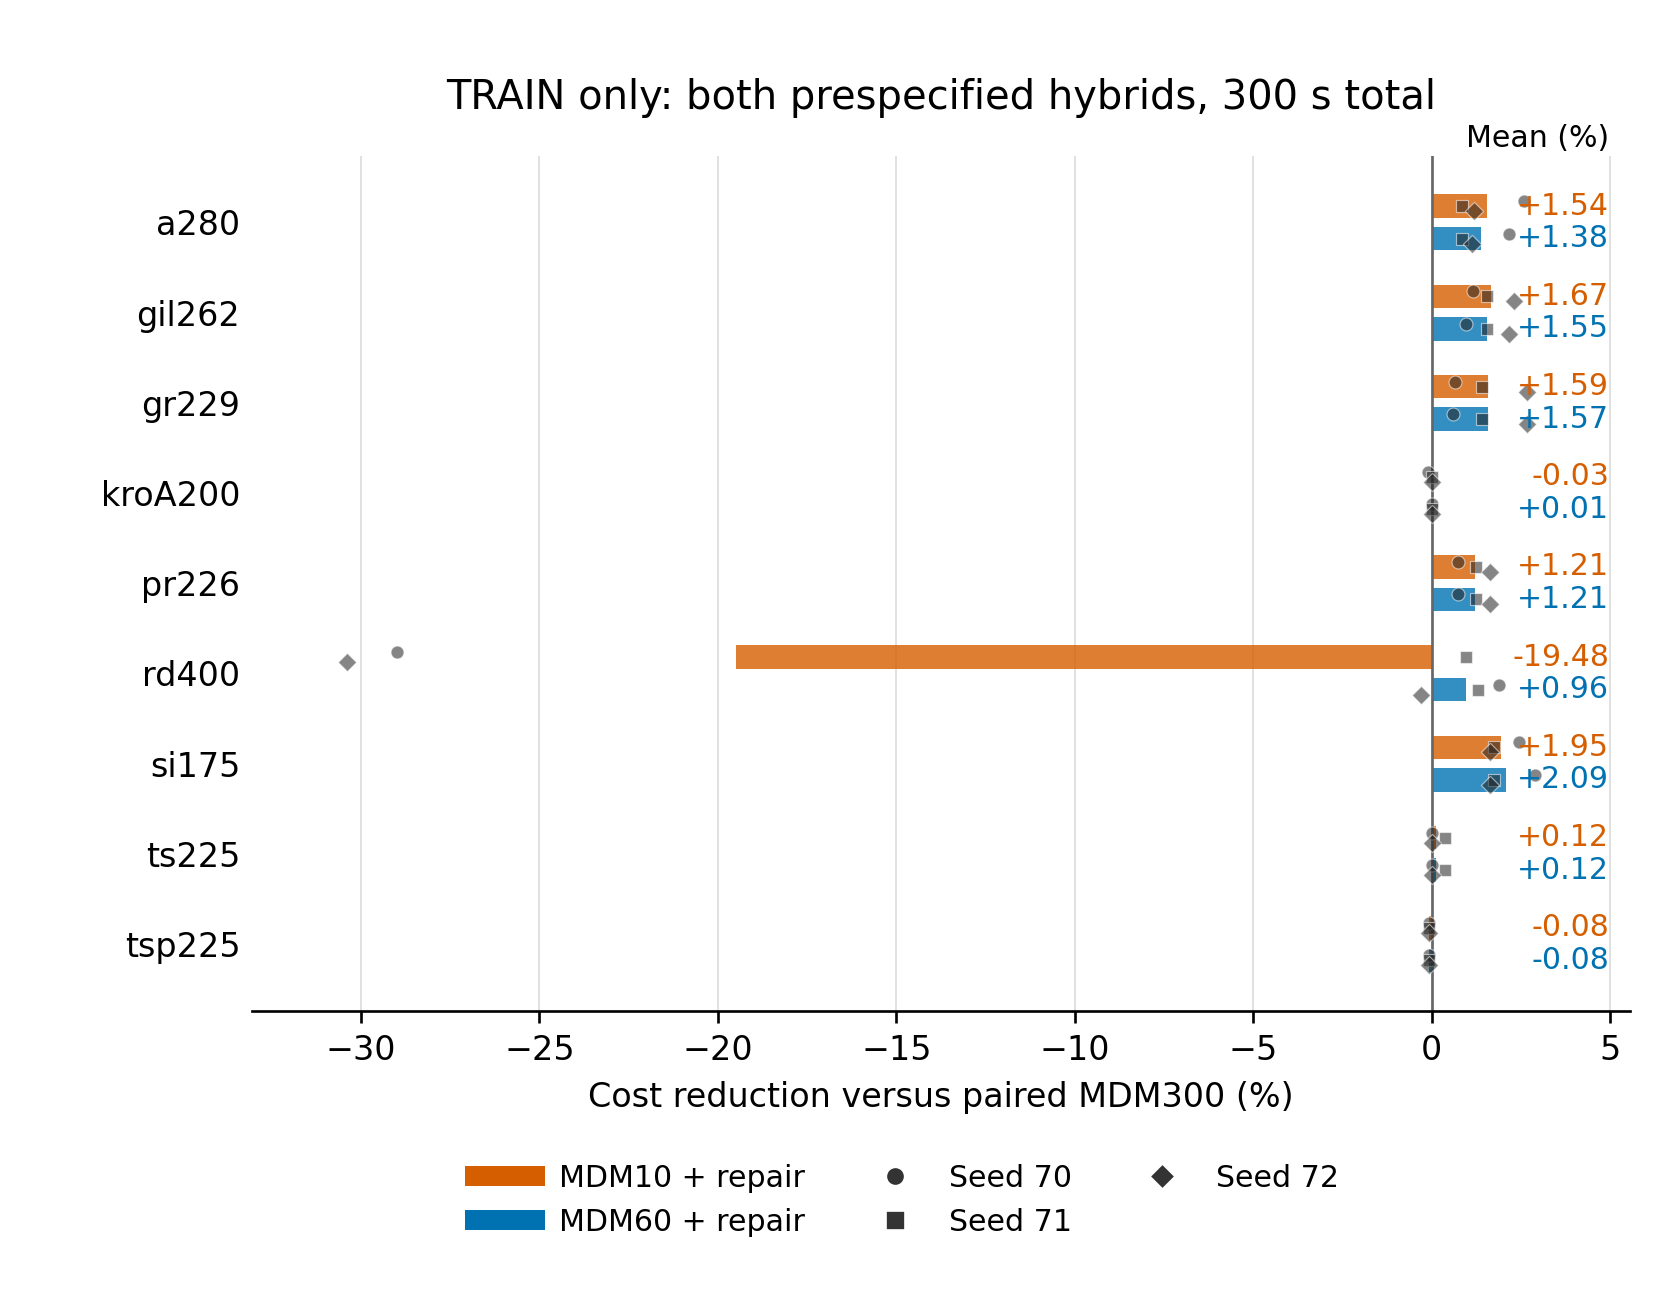
\includegraphics[width=\textwidth]{figures/awake300_effects.png}
\caption{Completed 300-second screen on nine selected TRAIN geometries and
three paired seeds. Bars show relative reductions of seed-mean costs;
markers show individual seed-pair reductions, not confidence intervals.
Both variants use the same horizontal axis and include initialization in
the total budget. Positive values favor the hybrid. The right-hand labels
give the geometry means. All losses are retained. This screen does not
establish performance on reserved test geometries or superiority over a
completed 70-iteration MDM reference.}
\label{fig:awake300-effects}
\end{figure}

Passive mining exports also qualify the comparison. MDM300 recorded mining
calls in 11 of its 27 executions; nine executions had a call provably within
the deadline. The 60-second hybrid initialization recorded calls in two
executions, one provably timely; the 10-second initialization recorded none.
These are bounds derived from available cumulative exports, not estimates
of the improvement caused by mining. The completed screen therefore supports
continued evaluation of the 60-second hybrid within the selected training
set. It does not replace the iteration-limited reference comparison.
